\documentclass{llncs}
%
%

\usepackage[dvips]{graphicx}
\usepackage{makeidx}  % allows for indexgeneration
\usepackage{amsmath}
\usepackage{amsfonts}

\hyphenation{pro-per-ties}
\hyphenation{ge-ne-ral-ly}
\hyphenation{pre-fe-ren-ces}
\hyphenation{u-sing}
\hyphenation{pu-nish-ment}

\newcommand{\Pow}{\mathcal{P}}
\newcommand{\N}{\operatorname{N}}
\newcommand{\bool}{\operatorname*{\mathcal{B}}}
\newcommand{\Pos}{\operatorname{Pos}}
\newcommand{\Nec}{\operatorname{Nec}}
\newcommand{\T}{\mathcal{T}}
\begin{document}

\mainmatter              % start of the contributions
%
\title{A possibilistic valid-time model}
%
%\titlerunning{A Fuzzy Valid-Time Model}  % abbreviated title (for running head)
%                                     also used for the TOC unless
%                                     \toctitle is used
%
\author{Jos\'e Enrique Pons \and Christophe Billiet \and Olga Pons Capote \and Guy de Tr\'e}
%Jeffrey Dean \and David Grove \and Craig Chambers \and Kim~B.~Bruce \and
%Elsa Bertino}
%
\authorrunning{Jos\'e Enrique Pons et al.} % abbreviated author list (for running head)
%
%%%% list of authors for the TOC (use if author list has to be modified)
%\tocauthor{Ivar Ekeland, Roger Temam, Jeffrey Dean, David Grove,
%Craig Chambers, Kim B. Bruce, and Elisa Bertino}
%
\institute{
Department of Computer Science and Artificial Intelligence \\
Universidad de Granada \\
Escuela T\'ecnica Superior de Ingenier\'ia Inform\'atica \\
C/Periodista Daniel Saucedo Aranda s/n \\
E-18071 (Granada-Spain)\\
\email{jpons,opc@decsai.ugr.es}\\ 
%WWW home page:
%\texttt{http://users/\homedir iekeland/web/welcome.html}
%\and
%Universit\'{e} de Paris-Sud,
%Laboratoire d'Analyse Num\'{e}rique, B\^{a}timent 425,\\
%F-91405 Orsay Cedex, France
\and 
Department of Telecommunications and Information Processing
Ghent University
Sint Pietersniewstraat 41 B-9000, Gent, Belgium.
\email{Christophe.Billiet,Guy.De.Tre@ugent.be}
}

\maketitle              % typeset the title of the contribution

\begin{abstract}

\end{abstract}

%
\section{Introduction}
\label{sec:Introduction}
Information systems (IS) have always tried to model parts of reality. To achieve this modelling, such systems contain data representing properties of real-world objects or concepts~\cite{JoseEnriquePons2012},~\cite{Billiet2012}. As time is an essential aspect of many real-world objects or concepts, information systems often contain data representing temporal notions which describe such temporal properties~\cite{Bolour1982},~\cite{VanderCruyssen1997}. Such temporal notions usually take the form of either instants~\cite{Jensen1998}, which can informally be seen as infinitely short `moments' or `points' in time, or time intervals~\cite{Jensen1998}.

Data are often produced by humans, but human-made data are prone to imperfections: some data may be vague, imprecise, incomplete, contradictory or uncertain. Data representing temporal notions may contain such imprecisions too~\cite{Devos1994},~\cite{Dubois2003},~\cite{JoseEnriquePons2012},~\cite{Billiet2012}. The work presented in this paper is specifically concerned with time intervals (and as a special case: instants) subject to uncertainty.

Generally, one of the most important purposes of an IS is to allow the retrieval of information or knowledge deduced from its data. Information or knowledge is usually retrieved from an IS by querying it and examining or analyzing the query results or by visualizing the contents of the IS, querying this visualization and examining or analyzing the resulting visualization(s).

Of course, when temporal information is represented in an IS, querying this IS may have a temporal aspect too. Usually, querying an IS containing data representing temporal notions is conceptually done by specifying one or more time indications and requesting information that is in a specific relationship with these indications, where the semantics of these relationships are specifically temporal~\cite{Billiet2012},~\cite{JoseEnriquePons2012},~\cite{Pons2012a}. Thus, some existing proposals have considered groups of basic relationships between time indications used to construct and express specific temporal relationships~\cite{Medina1994},~\cite{Schockaert2008}. Notably, Allen~\cite{Allen1983} presented a reasoning framework containing all semantically usefull basic temporal relationships between time intervals (and as a special case instants). The resulting relationships are shown in figure \ref{fig:allen-relationships}. These Allen relationships are used in the presented work.

\begin{figure}[h]
   \centering
   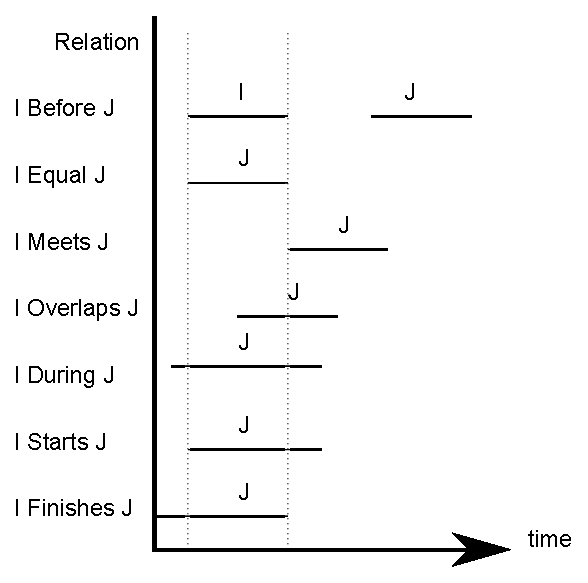
\includegraphics[width=0.9\columnwidth]{graphs/allen.eps}
   \caption{The Allen relationships between two crisp intervals $I$ and $J$.  }
   \label{fig:allen-relationships}
 \end{figure}

To be able to query IS containing data representing time indications subject to uncertainty, a framework is necessary, able to represent uncertainties in time indications in a semantically sound way, without (much) information loss and able to temporally reason with such time indications in a semantically sound and usefull way~\cite{Dubois1983},~\cite{Dubois2003}. Although more proposals for such frameworks exist, the work presented in this paper focusses on just two: the \emph{ill-known constraint \emph{(IKC)} framework}~\cite{Pons2011} and the \emph{triangular model \emph{(TM)} framework}~\cite{DeTre2012}.

The work presented in this paper consists of a comparison of both frameworks, about the approaches they use to represent time intervals subject to uncertainty and to reason about the temporal relationships between such intervals and time intervals without uncertainty.

The structure of this paper is as follows: section \ref{sec:general-preliminaries} presents some general preliminaries and naming and notation conventions used in this paper. Sections \ref{sec:ikc} and \ref{sec:tm} introduce the IKC and TM frameworks respectively: both sections first introduce some preliminary concepts and techniques specific to the framework under consideration, then explain how the representation of time intervals by the framework is done and finally show how the evaluation of Allen relationships between an interval subject to uncertainty and one without uncertainty is done. In section \ref{sec:proposal}, both frameworks are compared: first their approaches to representing time intervals are compared, next their approaches to evaluating Allen relationships are compared. Finally, section \ref{sec:conclusions} presents the principal conclusions of the presented work and some possible future work. 

%TODO: more references in the above part?
%TODO: include some form of proof or previous work with these statements?!

%The concept of the time has been widely studied \cite{Benthem1982}, \cite{Shackle1961}, \cite{Klein1994}. Moreover, humans beings manage temporal indications in an imprecise way \cite{Devos1998}. But when dealing with time in an Information System, some simplifications must to be done. The first thing to do is the discretization of the time line into time points or time intervals. Both approaches have been proved to be equivalent, although due to the nature of the smallest unit of time in a computer, a \emph{chronon}, the discretization of a time point returns a time interval.

%All the possible positions between two time intervals were studied by Allen \cite{Allen1983}, \cite{Allen1985}. As result, the thirteen Allen's Relations were obtained (See Table \ref{tab:allen-relations}) which are illustrated in Figure \ref{fig:allen-relationships}. In order to achieve a more intelligent processing of time, some theoretical frameworks are used to reason with time. First the possibility theory was employed in the reasoning with temporal information \cite{Dubois2003a}. Then, several proposals \cite{Schockaert2008}, \cite{nagypal2003}, \cite{Ohlbach2004}, \cite{Pons2011} studied how to extend the thirteen Allen's relations to the possibilistic case. Also rough set theory \cite{Pawlak1995} has been used to represent and reason about imperfect time intervals \cite{Qiang2009}, \cite{Qiang2010}.

%Although there exists several proposals to represent and visualize imperfect time intervals, in this paper we will focus on two: the ill-known constraint framework \cite{Pons2011} and the triangular model \cite{DeTre2012}. The first one is a theoretical framework that deals with temporal reasoning and the second one is a visual framework that represent imperfect time intervals in a two dimensional space. Both frameworks can be used to represent imperfect time intervals as well as temporal reasoning.

%The structure of this paper is the following. Section  \ref{sec:preliminaries} introduces the Ill-known constraint framework. Section \ref{sec:triangular-model} introduces the triangular model. Section \ref{sec:proposal} analyze both frameworks and shows the correspondences and differences between both frameworks. The section concludes with an example showing that the calculations made in both frameworks are equivalent. Finally, Section \ref{sec:conclusions} presents the main conclusions and the future work. 


%\begin{table}[h]
%\centering
%\begin{tabular}{|c|l|}
%\hline
%Name & Implementation \\ \hline 
%$I$ equals $J$ & if $s_i = s_j \wedge e_i = e_j $ \\
%$I$ starts $J$ & if $s_i = s_j \wedge e_i < e_j $ \\
%$I$ started by $J$ & if $s_i = s_j \wedge e_i > e_j $ \\
%$I$ finishes $J$ & if $s_i > s_j \wedge e_i = e_j $ \\
%$I$ finished by $J$ & if $s_i < s_j \wedge e_i = e_j $ \\
%$I$ meets $J$ & if $e_i = s_j $ \\
%$I$ met by $J$ & if $s_i = e_j $ \\
%$I$ overlaps $J$ & if $s_i < s_j \wedge e_i < e_j \wedge e_i > s_j $ \\
%$I$ overlapped by $J$ & if $s_i > s_j \wedge e_j < e_i \wedge s_i < e_j  $ \\
%$I$ during $J$ & if $s_i > s_j \wedge e_i < e_j $ \\
%$I$ contains $J$ & if $  s_i < s_j \wedge e_i > e_j$ \\
%$I$ before $J$ & if $e_i < s_j $ \\
%$I$ after $J$ & if $s_i > e_j $ \\
%\hline
%\end{tabular}
%\caption{Allen's relations represented in the framework. $I = \left[s_i, e_i\right]$, $J=  \left[s_j, e_j\right]$}
%\label{tab:allen-relations}
%\end{table}


%

\section{Preliminaries}
\label{sec:preliminaries}
%Introductory text:
In this section, we introduce some basic concepts concerning possibilistic variables and fuzzy numbers and intervals. Then, the framework of set evaluation by ill-known constraints \cite{Pons2011} is explained. The section concludes with a brief introduction to temporal databases.


% %Something about relational databases in general and relations in specific (to make the vocabulary clear)
% \subsection{Relational Databases}
% In this subsection, a few structural and behavioral aspects of the relational database model will be presented.
% 
% In a relational database, information is structured in \emph{relations}. As explained in the introduction, a collection of similar entities is modelled by an entitytype, which, using the relational database model, will be modelled by a relation. A relation consists of a \emph{relation schema} and an \emph{extention}. The relation schema basically determines the relation structure, by dictating which data (describing entities) will be kept and how these data will be represented. Each (atomic) part of these data is a result value of a measurement of a property of an entity or a description of a property of an entity. The extention contains these data. A relation schema consists of a \emph{relation name} and a finite set of \emph{attributes}. The relation name is of course the name of the entire relation, while the attributes describe common properties of the entities modelled by the relation. Every attribute consists of an attribute name and an associated \emph{data type}. Each data type has its \emph{domain} and its operators. The domain of a data type is the set of values which data of the data type in question can assume. Operators of a data type can be applied to data of a data type. The extention of a relation is a set of \emph{tuples}. Each tuple represents an enitity, by containing values: for every attribute in the attribute set of the relation schema, the tuple contains the value describing the exact state of the property of the entity. %Remember: a tuple is just an ordered tuple of values.

\subsection{\label{subsec:possibility-theory}Possibility Theory}
Possibility theory is devoted to the handling of incomplete information. In order to capture partial ignorance, two measures are provided: possibility and necessity.

\begin{definition}
Consider a set of outcomes $\Omega$. Let $\wp(\Omega)$ denote the powerset of $\Omega$ and let $A$ and $B$ be elements of $\wp(\Omega)$. A \emph{confidence measure on $\Omega$} is defined by a function
	\begin{align}
	g : \wp(\Omega) & \rightarrow \left[0,1\right]
	\end{align}
that satisfies
	\begin{align}
	g(\emptyset) &= 0 \\
	g(\Omega) &= 1 	\label{NormalizationProperty} \\
	A \subseteq B &\Rightarrow g(A) \leq g(B) \label{MonotonicityProperty}
	\end{align}
\end{definition}

Both possibility and necessity measures are special cases of confidence measures.



\begin{definition}
Consider a confidence measure $\Pi$ on a set of outcomes $\Omega$. Let $J$ be a countable index set and let $\{ A_{j} | j \in J \wedge A_{j} \subseteq \Omega \}$ be a family of elements of $\wp(\Omega)$. $\Pi$ is now a \emph{possibility measure on $\Omega$} if it satisfies:
	\begin{align}
	\Pi\left(\bigcup_{j \in J} A_{j} \right) = \sup_{j \in J} \Pi(A_{j})
	\end{align}
\end{definition}

In this work, the interpretation is as follows. The possibility of an event expresses how plausible the occurrence of the event seems to an observer of the experiment, given the (partial) knowledge of the observer about the experiment.

Information on the possibility of distinct elements of the universe of discourse $\Omega$ can now be given by a \emph{possibility distribution} $\pi$ on $\Omega$, defined by:

\begin{definition}
Consider a possibility measure $\Pi$ on $\Omega$. A \emph{possibility distribution} $\pi$ on $\Omega$ underlying the possibility measure $\Pi$ is a function defined by:
	\begin{align}
	\pi : \Omega \rightarrow \left[0, 1\right] : \pi(u) = \Pi(\{u\})
	\end{align}
\end{definition}

\begin{definition}
Consider a confidence measure $N$ on $\Omega$. Let $J$ be a countable index set and let $\{ A_{j} | j \in J \wedge A_{j} \subseteq \Omega \}$ be a family of elements of $\wp(\Omega)$. $N$ is a \emph{necessity measure} on $\Omega$ if it satisfies:
	\begin{align}
	N\left(\bigcap_{j \in J} A_{j} \right) = \inf_{j \in J} N(A_{j})
	\end{align}
\end{definition}

In this work, the interpretation is as follows. The necessity of an event expresses how necessary the occurrence of the event seems to an observer of the experiment, given the (partial) knowledge of the observer about the experiment.

Possibility and necessity measures are dual in the sense that:

\begin{align}
\forall A \subseteq \Omega : N(A) = 1 - \Pi(\bar{A})
\end{align}

That is, the degree to which an event is necessary is the extent to every other possible event is not plausible.

\subsection{\label{subsec:possibilistic-variables}Possibilistic Variables}
Possibilistic variables rely on possibility theory \cite{Dubois1988a} and are defined as follows \cite{Pons2011}.

\begin{definition}
\label{def;possibilistic-variable}
A possibilistic variable $X$ over a universe $U$ is defined as a variable taking exactly one value in $U$, but for which this value is (partially) unknown. Possibility distribution $\pi_X$ on $U$ models the available knowledge about the value $X$ takes; for each $u\in U$, $\pi_X(u)$ represents the possibility that $X$ takes the value $u$. In this work, this possibility is interpreted as a measure of how plausible it is that $X$ takes the value $u$, given (partial) knowledge about the value $X$ takes.
\end{definition}

The exact value a possibilistic variable takes, which is (partially) unknown, is called an \emph{ill-known value} in this work \cite{Dubois1988a}.

When a possibilistic variable is defined on the powerset $\Pow(U)$ of some universe $U$, the unique value the variable takes will be a crisp set and its possibility distribution on the powerset $\Pow(U)$ will describe the possibility of each crisp subset of $U$ to be the value the variable takes. This exact value (a crisp set) the variable takes, is now called an \emph{ill-known set} \cite{Dubois1988a}.

% It is important to understand the difference between the following two concepts:
% \begin{itemize}
% \item
% A \emph{possibilistic variable} $X$ is bounded to take only one value , but this value is not known due to incomplete knowledge. 
% \item
% An \emph{ill-known set}~\cite{Dubois1988a}: a possibilistic variable defined over the universe $\Pow(U)$.
% \end{itemize}

Note that while a possibilistic variable refers to one (partially) unknown value, an ill-known set is a crisp set but, for some reason, (partially) unknown.

A specific application of possibilistic variables is obtained when the universe under consideration is the set of Boolean values $\mathbb{B}$ = $\{T,F\}$. Indeed, any Boolean proposition $p$ takes just one value in $\mathbb{B}$. If the knowledge about which value this proposition $p$ will take is given by a possibility distribution $\pi_p$; the proposition can be seen as a possibilistic variable. The possibility and necessity that $p$ = $T$ (the proposition holds) demand more attention. This possibility and necessity is noted here as:
\begin{align}
\label{propholdsposs}
\text{Possibility that $p$ = $T$ (p holds):} &\\
\nonumber
Pos(p) = \pi_p(T)  \\
\label{propholdsnecc}
\text{Necessity that $p$ = $T$ (p holds):} & \\
\nonumber
Nec(p) = 1-\pi_p(F) 
\end{align}

Here, equation \eqref{propholdsposs} denotes the possibility that $p$ = $T$ and the proposition holds, while equation \eqref{propholdsnecc} denotes the necessity that $p$ = $T$ and the proposition holds.

This work deals with ill-known intervals. These are ill-known sets, defined and represented via a starting and ending points that, in turn are ill-known values. The elements of the set are the values between the starting and ending points. A closed ill-known interval with starting point defined by possibilistic variable $X$ and ending point by possibilistic variable $Y$ is noted here $\left[X, Y\right]$. %The correspondences and transitions between the representations of ill-known sets, between the representations of ill-known intervals and between the representations of an ill-known set and an ill-known interval are part of the authors current research.

\subsection{\label{subsec:fuzzy-numbers}Fuzzy Numbers and Fuzzy Intervals}
Among others, Dubois and Prade~\cite{Dubois1983} use fuzzy sets \cite{Zadeh1965} to define a \emph{fuzzy interval}:
\begin{definition}
A fuzzy interval is a fuzzy set $M$, defined by a membership function $\mu_{M}$ on the set of real numbers $\mathbb{R}$ such that:
\begin{eqnarray}
\mu_{M} :  \mathbb{R} \rightarrow \left[0,1\right]  \\ 
\nonumber
\forall (u,v)\in\mathbb{R}^2: \forall w \in [u,v]:\\
\nonumber
\mu_M(w) \geq\min(\mu_M(u),\mu_M(v))  \\
\nonumber
\exists m \in \mathbb{R} :  \mu_M(m)=1 
\end{eqnarray}
\end{definition}

\begin{samepage}
\vspace*{13pt}
\begin{center}
{
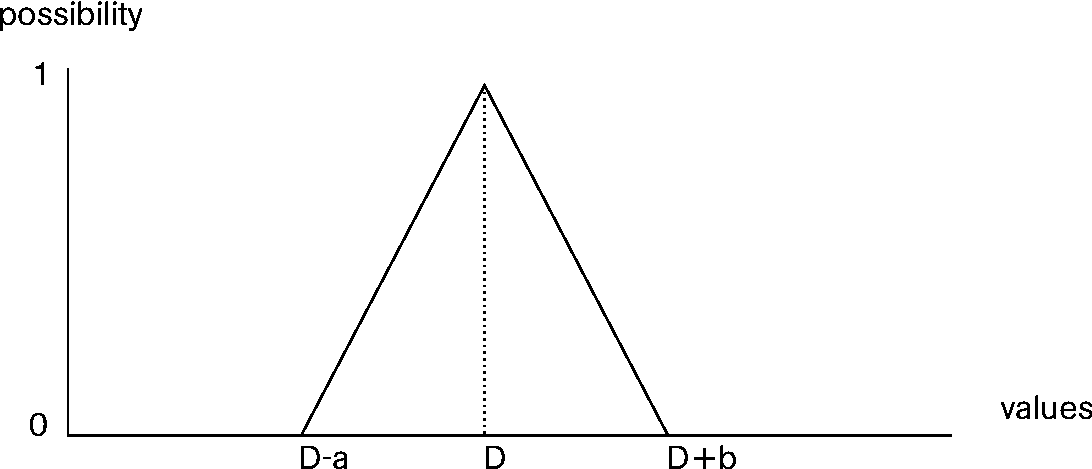
\includegraphics[scale=0.25]{./graphs/triangular.pdf}

}
\end{center}
%\centerline{ 
\psfig{file=./graphs/Y-time-point.eps}}
\vspace*{10pt}
\fcaption{\label{fig:triangular-dist}Example of fuzzy number.}
%  \label{fig:fuzzy-validity-period}
\vspace*{13pt}
\end{samepage}
If this modal value $m$ is unique, then $M$ is referred to as a \emph{fuzzy number}. 
%In other words, if the core of a fuzzy interval is a singleton, it is referred to as a fuzzy number (Figure \ref{fig:triangular-dist}).

A simple form of the membership function of a fuzzy interval is a trapezoidal function (Figure \ref{fig:trapezoidal-dist}). It can be shown that such a membership function $\mu_T$ for a fuzzy interval $T$ is convex and normalized. The values $\left[\alpha, \beta, \gamma, \delta\right]$ represent a trapezoidal possibility distribution defined by $\mu_T$:

% Four real values, denoted $\alpha$, $\beta$, $\gamma$ and $\delta$ suffice to represent a trapezoidal membership function of a fuzzy interval. In this work, a fuzzy interval defined as such will be noted as . The corresponding membership function definition for this  is then given by:

\begin{align}
\mu_T : & \quad \mathbb{R} \rightarrow \left[0,1\right] \\
\nonumber
 : & \quad x \rightarrow
\begin{cases}
1 & \mbox{ if } x \in [\beta,\gamma] \\
0 & \mbox{ if } x > \delta \vee x < \alpha \\
\frac{x-\alpha}{\beta - \alpha} & \mbox{ if } x \in [\alpha,\beta[ \\
\frac{\delta -x}{\delta - \gamma} & \mbox{ if } x \in ]\gamma,\delta] \\
\end{cases}
\end{align}

\begin{samepage}
\vspace*{13pt}
\begin{center}
{
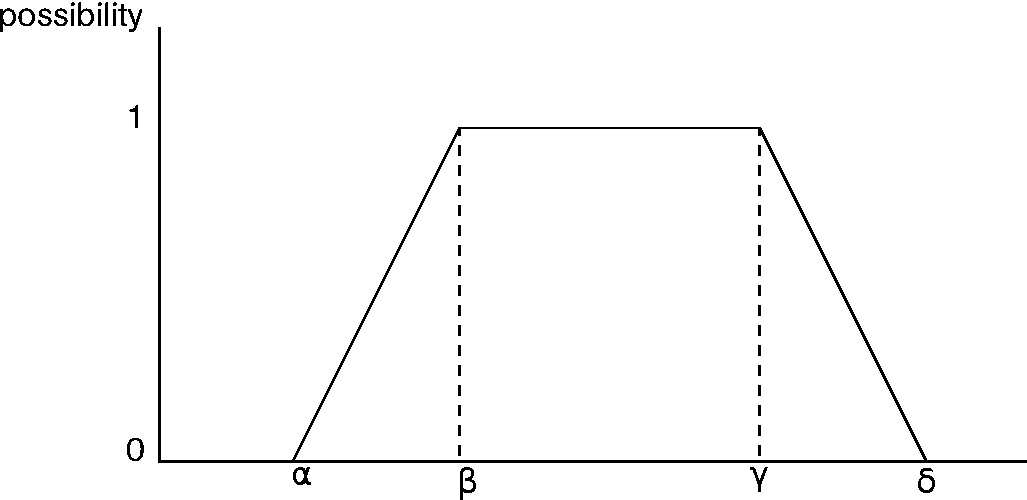
\includegraphics[scale=0.25]{./graphs/trapezoidalDistribution.pdf}

}
\end{center}
%\centerline{ 
\psfig{file=./graphs/Y-time-point.eps}}
\vspace*{10pt}
\fcaption{\label{fig:trapezoidal-dist}Example of fuzzy interval.}
%  \label{fig:fuzzy-validity-period}
\vspace*{13pt}
\end{samepage}

%\def\JPicScale{0.5}
%\begin{figure}[h!]
%  \centering
%  %%Created by jPicEdt 1.4.1_03: mixed JPIC-XML/LaTeX format
%%Thu Nov 17 17:57:10 CET 2011
%%Begin JPIC-XML
%<?xml version="1.0" standalone="yes"?>
%<jpic x-min="5" x-max="125" y-min="5" y-max="75" auto-bounding="true">
%<multicurve fill-style= "none"
%	 points= "(10,10);(10,10);(10,60);(10,60)"
%	 right-arrow= "head"
%	 />
%<multicurve fill-style= "none"
%	 points= "(10,10);(10,10);(110,10);(110,10)"
%	 right-arrow= "head"
%	 />
%<multicurve fill-style= "none"
%	 points= "(30,10);(30,10);(50,60);(50,60)"
%	 />
%<multicurve fill-style= "none"
%	 stroke-color= "#ccccff"
%	 points= "(70,60);(70,60);(90,10);(90,10)"
%	 />
%<text fill-style= "none"
%	 stroke-color= "#ff0033"
%	 stroke-width= "0.95"
%	 text-vert-align= "center-v"
%	 anchor-point= "(125,40)"
%	 text-frame= "noframe"
%	 text-hor-align= "center-h"
%	 >
%
%</text>
%<text fill-style= "none"
%	 stroke-color= "#ff0033"
%	 stroke-width= "0.95"
%	 text-vert-align= "center-v"
%	 anchor-point= "(30,5)"
%	 text-frame= "noframe"
%	 text-hor-align= "center-h"
%	 >
%$\alpha$
%</text>
%<text fill-style= "none"
%	 stroke-color= "#ff0033"
%	 stroke-width= "0.95"
%	 text-vert-align= "center-v"
%	 anchor-point= "(50,5)"
%	 text-frame= "noframe"
%	 text-hor-align= "center-h"
%	 >
%$\beta$
%</text>
%<text fill-style= "none"
%	 stroke-color= "#ff0033"
%	 stroke-width= "0.95"
%	 text-vert-align= "center-v"
%	 anchor-point= "(90,5)"
%	 text-frame= "noframe"
%	 text-hor-align= "center-h"
%	 >
%$\delta$
%</text>
%<text fill-style= "none"
%	 stroke-color= "#ff0033"
%	 stroke-width= "0.95"
%	 text-vert-align= "center-v"
%	 anchor-point= "(5,60)"
%	 text-frame= "noframe"
%	 text-hor-align= "center-h"
%	 >
%1
%</text>
%<text fill-style= "none"
%	 stroke-color= "#ff0033"
%	 stroke-width= "0.95"
%	 text-vert-align= "top"
%	 anchor-point= "(110,75)"
%	 text-rotation= "90"
%	 text-frame= "noframe"
%	 text-hor-align= "center-h"
%	 stroke-style= "dotted"
%	 >
%
%</text>
%<text fill-style= "none"
%	 text-vert-align= "center-v"
%	 anchor-point= "(45,70)"
%	 text-frame= "noframe"
%	 text-hor-align= "center-h"
%	 >
%
%</text>
%<text fill-style= "none"
%	 stroke-color= "#ff0033"
%	 stroke-width= "0.95"
%	 text-vert-align= "center-v"
%	 anchor-point= "(5,5)"
%	 text-frame= "noframe"
%	 text-hor-align= "center-h"
%	 >
%0
%</text>
%<text fill-style= "none"
%	 text-vert-align= "center-v"
%	 anchor-point= "(15,65)"
%	 text-frame= "noframe"
%	 text-hor-align= "center-h"
%	 >
%membership degree
%</text>
%<multicurve fill-style= "none"
%	 points= "(50,60);(50,60);(70,60);(70,60)"
%	 />
%<multicurve fill-style= "none"
%	 polydots-size-linewidth-scale= "2.5"
%	 polydots-style= "polydots-circle"
%	 stroke-color= "#3300cc"
%	 polydots-scale-v= "1"
%	 polydots-angle= "0"
%	 polydots-scale-h= "1"
%	 stroke-dasharray= "1;1"
%	 polydots-superimpose= "false"
%	 points= "(50,60);(50,60);(50,10);(50,10)"
%	 polydots-size-minimum= "0.7"
%	 stroke-style= "dashed"
%	 />
%<multicurve fill-style= "none"
%	 stroke-dasharray= "1;1"
%	 points= "(70,60);(70,60);(70,10);(70,10)"
%	 stroke-style= "dashed"
%	 />
%<text fill-style= "none"
%	 stroke-color= "#ff0033"
%	 stroke-width= "0.95"
%	 text-vert-align= "center-v"
%	 anchor-point= "(70,5)"
%	 text-frame= "noframe"
%	 text-hor-align= "center-h"
%	 >
%$\gamma$
%</text>
%</jpic>
%%End JPIC-XML
%LaTeX-picture environment using emulated lines and arcs
%You can rescale the whole picture (to 80% for instance) by using the command \def\JPicScale{0.8}
\ifx\JPicScale\undefined\def\JPicScale{1}\fi
\unitlength \JPicScale mm
\begin{picture}(125,75)(0,0)
\linethickness{0.3mm}
\put(10,10){\line(0,1){50}}
\put(10,60){\vector(0,1){0.12}}
\linethickness{0.3mm}
\put(10,10){\line(1,0){100}}
\put(110,10){\vector(1,0){0.12}}
\linethickness{0.3mm}
\multiput(30,10)(0.12,0.3){167}{\line(0,1){0.3}}
\linethickness{0.3mm}
\multiput(70,60)(0.12,-0.3){167}{\line(0,-1){0.3}}
\put(125,40){\makebox(0,0)[cc]{}}

\put(30,5){\makebox(0,0)[cc]{$\alpha$}}

\put(50,5){\makebox(0,0)[cc]{$\beta$}}

\put(90,5){\makebox(0,0)[cc]{$\delta$}}

\put(5,60){\makebox(0,0)[cc]{1}}

\put(110,75){\makebox(0,0)[tc]{}}

\put(45,70){\makebox(0,0)[cc]{}}

\put(5,5){\makebox(0,0)[cc]{0}}

\put(15,65){\makebox(0,0)[cc]{membership degree}}

\linethickness{0.3mm}
\put(50,60){\line(1,0){20}}
\linethickness{0.3mm}
\multiput(50,10)(0,1.96){26}{\line(0,1){0.98}}
\linethickness{0.3mm}
\multiput(70,10)(0,1.96){26}{\line(0,1){0.98}}
\put(70,5){\makebox(0,0)[cc]{$\gamma$}}

\end{picture}

%  \caption{Trapezoidal membership function}
%  \label{fig:trapezoidal}
%\end{figure}


The representation for a triangular possibility distribution is given by three values $\left[D,a,b \right]$. The distribution is obtained from a trapezoidal possibility distribution by replacing the values $\left[D-a, D, D, D+b \right]$.


% The most convenient form of the membership function of a fuzzy number is a triangular form. It can be shown that such a membership function $\mu_M$ for a fuzzy number $M$ is convex and normalized. Three real values, denoted by $a$, $b$ and $D$, suffice to represent a triangular membership function of a fuzzy number and in this work, a fuzzy number defined as such will be noted as $\left[D, a, b \right]$. Here:
% \begin{itemize}
% \item
% $D$ denotes the single value in the core of $M$
% \item
% $D-a$ is then $\inf \{u \in \mathbb{R} : \mu_{M}(u) > 0\}$
% \item
% $D+b$ is then $\sup \{u \in \mathbb{R} : \mu_{M}(u) > 0\}$
% \end{itemize}
% 
% The membership function of such a fuzzy number is then given by:
% 
% \vspace{-10pt}
% 
% \begin{align}
% \mu_M :   \mathbb{R} \rightarrow \left[0,1\right] :  x \rightarrow \nonumber\\
% \begin{cases}
% \nonumber
% 0 & \mbox{ if } \left(x < D-a\right) \vee \left(x > D+b\right) \\
% \frac{\left[x-\left(D-a\right)\right]}{a} & \mbox{ if } \left(x \geq D-a\right) \wedge (x \leq D)  \\
% -\frac{\left[x-\left(D+b\right)\right]}{b} & \mbox{ if } \left(x \geq D\right) \wedge (x \leq D+b)
% \end{cases}
% \end{align}

%\begin{figure}[h!]
%  \centering
%  %%Created by jPicEdt 1.4.1_03: mixed JPIC-XML/LaTeX format
%%Thu Jan 12 17:26:56 CET 2012
%%Begin JPIC-XML
%<?xml version="1.0" standalone="yes"?>
%<jpic x-min="-2.5" x-max="60" y-min="-2" y-max="32.5" auto-bounding="true">
%<multicurve right-arrow= "head"
%	 fill-style= "none"
%	 points= "(0,0);(0,0);(55,0);(55,0)"
%	 />
%<multicurve right-arrow= "head"
%	 fill-style= "none"
%	 points= "(0,0);(0,0);(0,30);(0,30)"
%	 />
%<text right-arrow= "head"
%	 fill-style= "none"
%	 text-vert-align= "center-v"
%	 anchor-point= "(-2.5,27.5)"
%	 text-frame= "noframe"
%	 text-hor-align= "center-h"
%	 >
%1
%</text>
%<text right-arrow= "head"
%	 fill-style= "none"
%	 text-vert-align= "center-v"
%	 anchor-point= "(-2.5,0)"
%	 text-frame= "noframe"
%	 text-hor-align= "center-h"
%	 >
%0
%</text>
%<text right-arrow= "head"
%	 fill-style= "none"
%	 text-vert-align= "center-v"
%	 anchor-point= "(15,32.5)"
%	 text-rotation= "135"
%	 text-frame= "noframe"
%	 text-hor-align= "center-h"
%	 >
%Membership Degree
%</text>
%<multicurve fill-style= "none"
%	 points= "(4,0);(4,0);(15,27.5);(15,27.5)"
%	 />
%<multicurve fill-style= "none"
%	 points= "(15,27.5);(15,27.5);(42,0);(42,0)"
%	 />
%<text fill-style= "none"
%	 text-vert-align= "center-v"
%	 anchor-point= "(60,0)"
%	 text-frame= "noframe"
%	 text-hor-align= "center-h"
%	 >
%Time
%</text>
%<text fill-style= "none"
%	 text-vert-align= "center-v"
%	 anchor-point= "(16,-2)"
%	 text-frame= "noframe"
%	 text-hor-align= "center-h"
%	 >
%$D$
%</text>
%<text fill-style= "none"
%	 text-vert-align= "center-v"
%	 anchor-point= "(4,-2)"
%	 text-frame= "noframe"
%	 text-hor-align= "center-h"
%	 >
%$D-a$
%</text>
%<text fill-style= "none"
%	 text-vert-align= "center-v"
%	 anchor-point= "(42,-2)"
%	 text-frame= "noframe"
%	 text-hor-align= "center-h"
%	 >
%$D+b$
%</text>
%</jpic>
%%End JPIC-XML
%LaTeX-picture environment using emulated lines and arcs
%You can rescale the whole picture (to 80% for instance) by using the command \def\JPicScale{0.8}
\ifx\JPicScale\undefined\def\JPicScale{1}\fi
\unitlength \JPicScale mm
\begin{picture}(60,32.5)(0,0)
\linethickness{0.3mm}
\put(0,0){\line(1,0){55}}
\put(55,0){\vector(1,0){0.12}}
\linethickness{0.3mm}
\put(0,0){\line(0,1){30}}
\put(0,30){\vector(0,1){0.12}}
\put(-2.5,27.5){\makebox(0,0)[cc]{1}}

\put(-2.5,0){\makebox(0,0)[cc]{0}}

\put(15,32.5){\makebox(0,0)[cc]{Membership Degree}}

\linethickness{0.3mm}
\multiput(4,0)(0.12,0.3){92}{\line(0,1){0.3}}
\linethickness{0.3mm}
\multiput(15,27.5)(0.12,-0.12){225}{\line(0,-1){0.12}}
\put(60,0){\makebox(0,0)[cc]{Time}}

\put(16,-2){\makebox(0,0)[cc]{$D$}}

\put(4,-2){\makebox(0,0)[cc]{$D-a$}}

\put(42,-2){\makebox(0,0)[cc]{$D+b$}}

\end{picture}

%  \caption{Triangular membership function.}
%  \label{fig:triangular}
%\end{figure}



\subsection{\label{subsec:interval-evaluation-by-ill-known-constraints}Interval Evaluation by Ill-known Constraints}
In our case, we need to know if all points in a crisp interval $I$ reside between the boundaries of an ill-known interval $\left[ X , Y \right]$. To compute that, we introduce the concept of \emph{ill-known constraint}\cite{Pons2011}.




\begin{definition}
Given a universe $U$, an ill-known constraint $C$ on a set $A \subseteq U$ is specified by means of a binary relation $R \subseteq U^{2}$ and a fixed ill-known value denoted by its possibilistic variable $V$ over $U$, i.e.:
\begin{align}
\label{eq:ill-known-constraint}
C \triangleq (R,V)
\end{align}
Set $A$ satisfies the constraint if and only if:
\begin{align}
\forall a \in A : (a,V) \in R
\end{align}
\end{definition}

An example of an ill-known constraint is $C_{ex} = (<, X)$. Some set $A$ satisfies $C_{ex}$ if $\forall a \in A : a < X$, given the possibilistic variable $X$.

The satisfaction of a constraint $C \triangleq (R,V)$ by a set $A$ is still a Boolean matter, but due to the uncertainty about the ill-known value $V$, it can be uncertain whether $C$ is satisfied by $A$ or not \cite{Pons2011}. In fact, this satisfaction now behaves as a proposition. Based on the possibility distribution $\pi_{V}$ of $V$, the possibility and necessity that $A$ satisfies $C$ can be computed. This proposition can thus be seen as a possibilistic variable on $\mathbb{B}$. The required possibility and necessity are:

\vspace{-10pt}

\begin{align}
\label{ill-known-pos}\
\Pos(A\text{ satisfies }C) & =\\
\nonumber
\min_{a \in A}\left(\sup_{(a,w) \in R}\pi_{V}(w)\right) \\
\label{ill-known-nec}
\Nec(A\text{ satisfies }C) & =\\
\nonumber
\min_{a \in A}\left(\inf_{(a,w) \notin R} 1-\pi_{V}(w)\right) 
\end{align}

So far, we have shown how it can be verified whether a set satisfies or not an ill-known constraint. The interval evaluation problem is explained in a more general context in \cite{Pons2011}.

\begin{samepage}
\vspace*{13pt}
\begin{center}
{
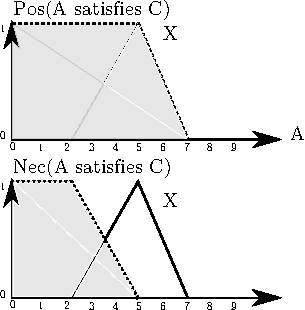
\includegraphics[scale=1]{./graphs/example-ill-known.pdf}
}
\end{center}
%\centerline{ 
\psfig{file=./graphs/Y-time-point.eps}}
\vspace*{10pt}
\fcaption{\label{fig:example-ill-known}Example of the evaluation of the ill-known constraint $C \triangleq (\leq, X), X = \left[5, 3, 2\right]$. Possibility and necessity measures are shown in grey. }
%  \label{fig:fuzzy-validity-period}
\vspace*{13pt}
\end{samepage}


\begin{example}
Consider  $X = \left[5, 3, 2 \right]$ and let $C =(\leq, X)$ the ill-known constraint. Then, the evaluation of the possibility and the necessity are obtained from \eqref{ill-known-pos} and \eqref{ill-known-nec} respectively. (See Figure \ref{fig:example-ill-known}).






 
\begin{align}
\Pos(A\text{ satisfies }C) & =\\
\nonumber
\min_{a \in A}\left(\sup_{a \leq w}\pi_{X}(w)\right)\\
\Nec(A\text{ satisfies }C) & =\\
\nonumber
\min_{a \in A}\left(\inf_{a > w} 1-\pi_{X}(w)\right) 
\end{align}




\end{example}





It is observed that Boolean combinations of constraints are required. For example, the problem of interval evaluation (explained earlier) requires that all the elements of an interval $[a,b]$ are larger than a value $X$ and, at the same time, smaller than a value $Y$, which implies that a conjunctive Boolean combination of both constraints must be satisfied. To allow Boolean combinations of constraints, the following definitions are introduced.
\begin{definition}
\label{def:set-evaluation}
Consider a universe $U$, an $n$-ary vector $\mathbf{C}$ of constraints and a Boolean function $\bool:\mathbb{B}^{n}\rightarrow\mathbb{B}$. An evaluation function is defined by:
\begin{equation}
\lambda:\Pow(U)\rightarrow\mathbb{B}:\lambda(A)\mapsto\bool\Big(C_{1}(A),...,C_{n}(A)\Big).
\end{equation}
\end{definition}
Definition \ref{def:set-evaluation} presents a function that evaluates a Boolean combination of some basic constraints. Informally, it states that a set $A$ passes the evaluation made by $\lambda$ if the Boolean combination of some propositions equals $T$. This crisp definition can be generalized to the case of ill-known constraints.
\begin{definition}
\label{def:ill-known-sets}
Consider a universe $U$, an $n$-ary vector $\mathbf{C}$ of ill-known constraints and a Boolean function $\bool:\mathbb{B}^{n}\rightarrow\mathbb{B}$. The uncertainty about the evaluation of a set $A$ by an evaluation function $\lambda$ is then given by:
\begin{equation}
\forall A\in\Pow(U):\pi_{\lambda(A)}=\widetilde{\bool}\Big(\pi_{C_1(A)},...,\pi_{C_n(A)}\Big)\\
\end{equation}
Hereby, $\widetilde{\bool}$ is the possibilistic extension of $\bool$.
\end{definition}
It is well known that any Boolean function $\bool$ can be cast to a canonical form~\cite{McCluskey1965}, requiring only logical conjunction $\wedge$, logical disjunction $\vee$ and logical negation. Therefore, only those connectives will be treated within the scope of this paper. By applying the possibilistic extensions of $\wedge$, $\vee$ and $\neg$, concrete equations are obtained for the calculations of uncertainty about the evaluation of a set by means of an evaluation function $\lambda$. In the case of conjunction (i.e., $\bool=\wedge$), the inference of uncertainty about the evaluation of a set reduces to:
\begin{eqnarray}
\label{eq:conjunctive1}
\forall A\in\Pow(U):\Pos(\lambda(A))&=\\
\nonumber
\min_{i=1 \ldots n}\Pos\left(C_i(A)\right)\\
\label{eq:conjunctive2}
\forall A\in\Pow(U):\Nec(\lambda(A))&=\\
\nonumber
\min_{i=1 \ldots n}\Nec\left(C_i(A)\right).
\end{eqnarray}
In the case of disjunction (i.e. $\bool=\vee$), the inference of uncertainty about the evaluation of a set reduces to:
\begin{eqnarray}
\label{eq:disjunctive}
\forall A\in\Pow(U):\Pos(\lambda(A))&=\\
\nonumber
\max_{i=1 \ldots n}\Pos\left(C_i(A)\right)\\
\forall A\in\Pow(U):\Nec(\lambda(A))&=\\
\nonumber
\max_{i=1 \ldots n}\Nec\left(C_i(A)\right).
\end{eqnarray}
Note that by using the functions $\min$ and $\max$ here, there is an implicit assumption that the possibilistic variables $\pi_{C_i}$ are mutual $\min$-dependent in the sense of De Cooman (i.e. non-interactive). For an extensive reading on (in)dependency of possibilistic variables, the reader is referred to~\cite{GertDeCooman1997b},\cite{GertDeCooman1997a},\cite{GertDeCooman1997}. In case of $\neg$, we get:
\begin{eqnarray}
\label{eq:negation}
\forall A\in\Pow(U):\Pos(\neg\lambda(A))&=\\
\nonumber
1-\Nec(\lambda(A))\\
\forall A\in\Pow(U):\Nec(\neg\lambda(A))&=\\
\nonumber
1-\Pos(\lambda(A)).
\end{eqnarray}

\begin{example}
Consider that we want to check if the crisp interval $I = \left[j, k\right]$ is included in $\left[X, Y\right]$. In this situation, two ill-known constraints are constructed.

%We assume that $X$ specifies the lower bound and $Y$ the upper bound for a given interval, we want to known whether all points in the interval are larger than or equal to $X$ and smaller than or equal to $Y$. Therefore, we consider two ill-known constraints:

\vspace{-10pt}

\begin{eqnarray}
\label{eq:constraint-c1}
C_1 & \triangleq\left(\geq,X\right)\\
\label{eq:constraint-c2}
C_2 & \triangleq\left(\leq,Y\right)
\end{eqnarray}

To calculate the possibility and necessity concerning a conjunction of constraints, the $\min$ operator can be used. The possibility and necessity of $I$ being included in $\left[X, Y\right]$ are now: %satisfying both constraints is then:

\vspace{-10pt}

\begin{align}
\label{eq:interval-pos}
\Pos(I\text{ satisfies }C_1\ and\ C_2) & =\\
\nonumber
\min_{a \in I}\left(\sup_{a \geq w}\pi_{X}(w),\sup_{a \leq v}\pi_{Y}(v)\right)\\
\label{eq:interval-nec}
\Nec(I\text{ satisfies }C_1\ and\ C_2) & =\\
\nonumber
\min_{a \in I}\left(\inf_{a < w} 1-\pi_{X}(w),\inf_{a > v} 1-\pi_{Y}(v)\right).
\end{align}
\end{example}

There is a special boolean combination of constraints that is of particular interest; let us see it.
\begin{definition}
\emph{Conjunctive combination of ill-known constraints}. Consider a universe $U$. Let $R_1, R_2$ be two binary relations in U. Let $X_1, X_2$ be two fixed ill-known values in $U$. Let  $C_1 = (R_1, X_1)$ and $C_2 = (R_2, X_2)$ be two ill-known constraints. A conjunctive combination of both constraints is given by:
\begin{align}
\label{eq:convex-combination}
CC \triangleq \left \lbrace C_1 \wedge C_2 \right \rbrace
\end{align}
In a more general way, it is possible to define the conjunctive combination of an n-ary vector of constraints:
\begin{align}
\label{eq:nary-convex-combination}
CC \triangleq \left \lbrace C_1 \wedge \ldots \wedge C_n \right \rbrace
\end{align}
\end{definition}

\begin{theorem}
\label{th:convex-combination-ill-known-constraints}
Consider the conjunctive combination $CC$ of any n-ary vector $\left \lbrace C_{1_{Z_1}}, \ldots, C_{n_{Z_n}} \right \rbrace$ of constraints over the ill-known variables $Z_1, \ldots, Z_n$. Then, if $\pi_{C_1(Z_1)}, \ldots, \pi_{C_n(Z_n)}$ are convex, then  $\pi_{CC}$ is also convex.
\end{theorem}

\begin{proof}
Let $CC \triangleq \left \lbrace C_{1_{Z_1}} \wedge \ldots \wedge C_{n_{Z_n}}  \right \rbrace$. Then:
\begin{align}
\label{eq:proof-convex1}
\pi_{CC} \left( \lambda x_1 + \left( 1 - \lambda \right)x_2 \right) = \\
\nonumber
\min  \big( \pi_{C_1(Z_1)}\left( \lambda x_1 + \left( 1 - \lambda \right)x_2 \right), \ldots,\\
\nonumber
   \pi_{C_n(Z_n)}\left( \lambda x_1 + \left( 1 - \lambda \right)x_2 \right)  \big)
\end{align}
Since $\pi_{C_1(Z_1)}, \ldots, \pi_{C_n(Z_n)}$ are convex:
\begin{align}
\label{eq:proof-convex2}
\pi_{C_1(Z_1)} \left(\lambda x_1 + \left( 1 - \lambda \right)x_2  \right) \geqq \\
\nonumber
\min \big(\pi_{C_1(Z_1)} \left( x_1 \right),\pi_{C_1(Z_1)} \left( x_2 \right)  \big)\\
\nonumber
\vdots \\
\nonumber
\pi_{C_n(Z_n)} \left(\lambda x_1 + \left( 1 - \lambda \right)x_2  \right) \geqq \\
\nonumber
\min \big(\pi_{C_n(Z_n)} \left( x_1 \right),\pi_{C_n(Z_n)} \left( x_2 \right) \big) 
\end{align}
Then, by using equation \eqref{eq:proof-convex1}:
\begin{align}
\label{eq:proof-convex3}
\pi_{CC} \left( \lambda x_1 + \left( 1 - \lambda \right)x_2 \right) \geqq  \\
\nonumber
\min \big( \min \left(\pi_{C_1(Z_1)} \left( x_1 \right),\pi_{C_1(Z_1)} \left( x_2 \right) \right),\\
\nonumber
\ldots, \min \left(\pi_{C_n(Z_n)} \left( x_1 \right),\pi_{C_n(Z_n)} \left( x_2 \right) \right) \big)
\end{align}
Which is equivalent to the following:
\begin{align}
\label{eq:proof-convex4}
\pi_{CC} \left( \lambda x_1 + \left( 1 - \lambda \right)x_2 \right) \geqq  \\
\nonumber
\min \big( \min \left(\pi_{C_1(Z_1)} \left( x_1 \right), \ldots, \pi_{C_n(Z_n)} \left( x_1 \right) \right),\\
\nonumber
\ldots, \min \left(\pi_{C_1(Z_1)} \left( x_2 \right), \ldots, \pi_{C_n(Z_n)} \left( x_2 \right) \right) \big)
\end{align}
Finally we obtain:
\begin{align}
\label{eq:proof-convex5}
\pi_{CC} \left( \lambda x_1 + \left( 1 - \lambda \right)x_2 \right) \geqq  \\
\nonumber
\min \big(\pi_{CC} \left( x_1 \right), \pi_{CC} \left( x_2 \right) \big)
\end{align}
\end{proof}

Sometimes, an ill-known value might be specified by a convex combination of ill-known constraints. This allow to define ill-known values by means of relationships with respect to other ill-known points.

%\begin{definition}
%\emph{Ill-known point defined by ill-known constraints}
%Consider a universe $U$, an n-ary vector $\mathbf{C}$ of ill-known constraints and a Boolean function $\bool:\mathbb{B}^{n}\rightarrow\mathbb{B}$. An ill-known value $X$ is defined by:
%\begin{align}
%\label{eq:ill-known-value-def-by-const}
%X \in \Pow(U):\pi_{X}=\widetilde{\bool}\Big(\pi_{C_1(Z_1)},...,\pi_{C_n(Z_n)}\Big)\\
%\end{align} 
%\end{definition}

\begin{definition}
\label{def:convex-combination-ill-known-constraints}
\emph{Ill-known value defined by conjunctive combination of constraints.}
Consider a universe $U$, $CC \triangleq \left \lbrace C_{1_{Z_1}} \wedge \ldots \wedge C_{n_{Z_n}}  \right \rbrace$ a conjunctive combination of ill-known constraints over the variables $Z_1, \ldots, Z_n$. The uncertainty about the evaluation of an ill-known value $X$ is given by:
\begin{align}
\label{eq:ill-known-value-def-by-const-unc}
X \in \Pow(U):\pi_{X}=\pi_{CC}
\end{align} 

The definition of the ill-known value $X$ with respect to the conjunctive combination of ill-known constraints, is written as:
\begin{align}
\label{eq:ill-known-value-by-convex-constraints}
X \triangleq CC 
\end{align}


Note that $\pi_{X}$ is convex since $\pi_{CC}$ is convex as demonstrated in Theorem \ref{th:convex-combination-ill-known-constraints}.
\end{definition}


\begin{example}
As an example, consider the hospital database. When a patient enters o leaves a medical service in hospital, a record tracking the patient is stored. The exact time for this is not precisely known. Consider now that $X = \left[12, 2, 2\right]$ is the time in hours when a patient left the emergency service and $Y = \left[18, 2, 1 \right]$ is the time in hours when the patient left the hospital. It is possible to obtain $Z$ (the period of time between the emergency service and the left of the patient) by using a conjunctive combination of constraints.

\begin{align}
\nonumber
CC = \left \lbrace C_1\left(>,X\right) \wedge C_2(\leq,Y) \right \rbrace \\
\nonumber
Z = CC
\end{align}
$Z$ is a fuzzy interval defined by a trapezoidal shape given by $\left[12,\ 14,\ 18,\ 19 \right]$.
Figure \ref{fig:example-ill-known-by-const} illustrates the relations among the variables $X$, $Y$ and $Z$.
\end{example}

\begin{samepage}
\vspace*{13pt}
\begin{center}
{
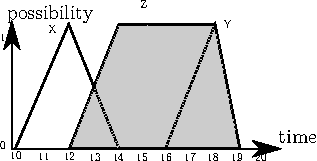
\includegraphics[scale=1]{./graphs/ill-known-by-constraints.pdf}

}
\end{center}
%\centerline{ 
\psfig{file=./graphs/Y-time-point.eps}}
\vspace*{10pt}
\fcaption{\label{fig:example-ill-known-by-const}Ill-known values $X$ and $Y$. The grey area represents the ill-known value $Z$ defined by the convex combination of the two ill-known constraints $C_1$ and $C_2$.}
\vspace*{13pt}
\end{samepage}

%\paragraph{Example} Consider the ill-known values $X = \left[5, 2, 8\right]$ and $Y = \left[9, 7, 10 \right]$. The knowledge about the evaluation of the interval $\left[a, b \right]$  is given by the expressions \eqref{eq:interval-pos},\eqref{eq:interval-nec}.  Figure~\ref{fig:3d-possibility} shows a 3D plot of the possibility that an interval $[a,b]$ passes the evaluations specified by the ill-known constraints. Note the triangular form for the resulting possibility distribution since the condition $a \leq b$ holds.
%
%\begin{figure}[h!]
%\centering
%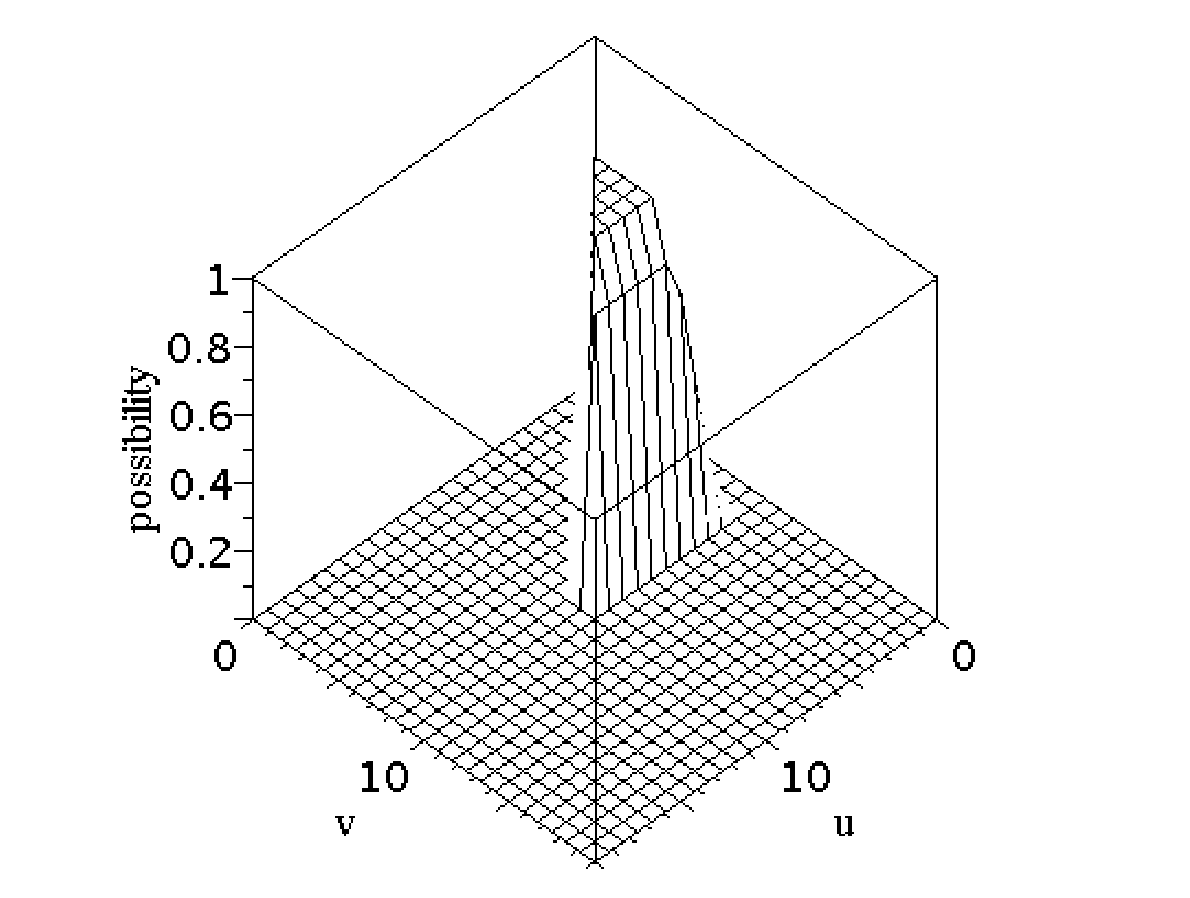
\includegraphics[scale=0.4]{graphs/3D_possibility.eps}
%\caption{Possibility of evaluation for the interval $[a,b]$.}
%\label{fig:3d-possibility}
%\end{figure}
%The necessity plot is obtained in a similar way and is shown in Figure~\ref{fig:3d-necessity}. Notice that the necessity measure is not normalized because the supports of $X$ and $Y$ overlap.
%\begin{figure}[h!]
%\centering
%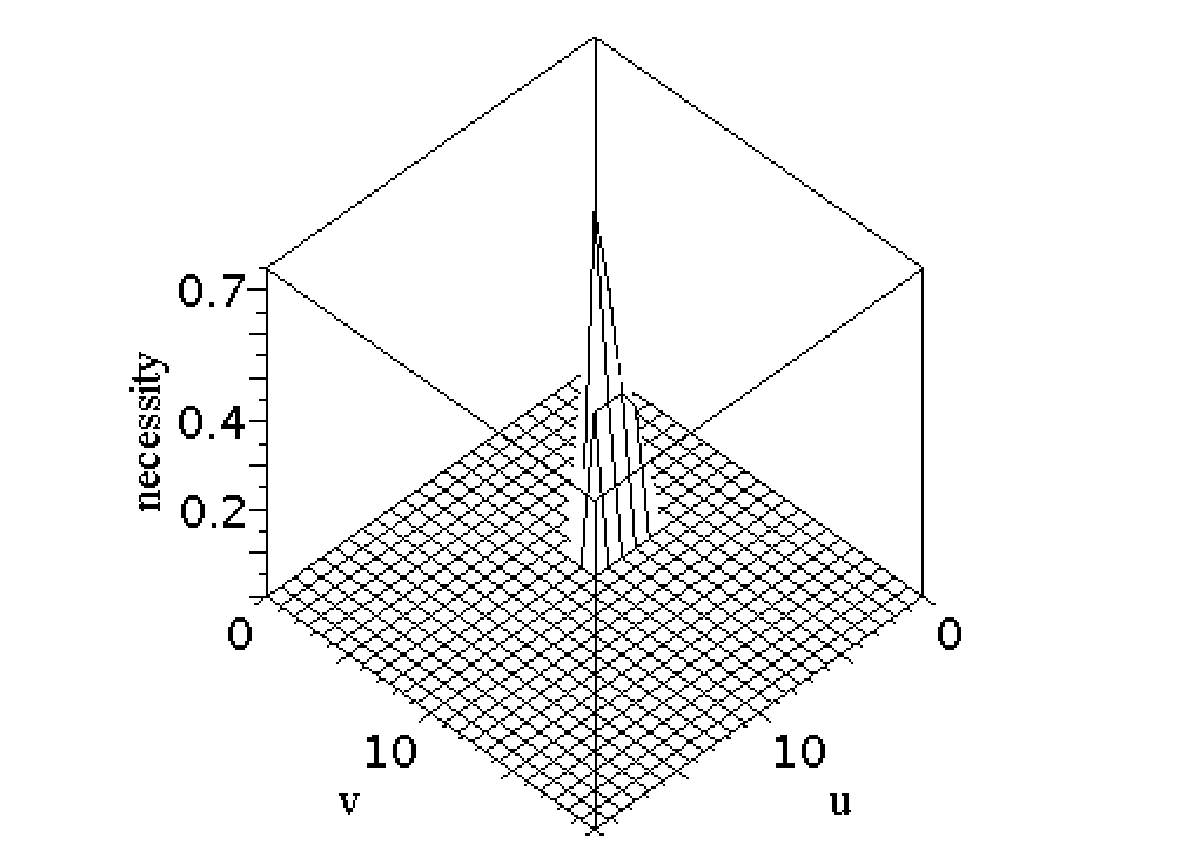
\includegraphics[scale=0.4]{graphs/3D_necessity.eps}
%\caption{Necessity of evaluation for the interval $[a,b]$.}
%\label{fig:3d-necessity}
%\end{figure}

%enlace:
We have seen the main theoretical concepts about ill-known values. Now, we are going to explain the main concepts about the treatment of time and the imperfection related to the time in databases. This two preliminary analysis will be the pillars of our proposal in section \ref{sec:time-rep}.

%In the following subsections we will show how to represent imperfect time intervals by means of ill-known values.






\section{Proposal}
\label{sec:proposal}
In this section, a valid-time model, able to handle imperfect valid-time notions, will be presented. First, the representation and storage of valid-time will be presented. Next, an approach to query the model is proposed. Finally, an example is given.
%The proposal consist on a possibilistic valid-time model. The representation and the querying are explained in the following subsections.

\subsection{Valid-time Intervals}
\subsubsection{Representation}
\label{subsec:representation-ill-known}
A database models real objects by storing the values of an object for each attribute describing a property of the object. Thus, a valid-time database following the presented proposal will model the time during which an object in a certain state is valid, by associating a \emph{Possibilistic Valid-time Period} (PVP) to the record describing this object state:

\begin{definition}
A \emph{Possibilistic Valid-time Period} is an ill-known interval in time, which models a time period during which an object in a certain state is valid.
\end{definition}

Because a PVP is an ill-known interval, it allows modelling the uncertainty about the start and/or end point of a time interval (and thus about the time interval itself) if such uncertainty exists. The interpretation is \emph{disjunctive}: the PVP represents exactly one valid-time interval, but precisely \emph{which} interval is represented, is (partially) unknown. In the presented model, only PVPs are considered of which the possibility distributions of the possibilistic variables defining the start and end point of the ill-known interval have exactly the same characteristics as the membership functions of fuzzy numbers. A perfectly known start or end point can then be modelled by such an ill-known value defined by a possibilistic variable $P$ for which $\exists ! x : \mu_{P}(x) > 0$.

As mentioned in \cite{Pon11}, this approach differs from the one where a valid-time period is represented by one fuzzy set. Such a fuzzy set is seen as a possibility distribution on $\mathbb{R}$ and thus defines just one ill-known value. However, in the presented approach, a time period is modelled using an ill-known set, which is defined by a possibility distribution on $\Pow(\mathbb{R})$.


%The interval has a starting and an ending points. An ill-known valid-time interval is an interval in witch one or both points are ill-known. 

%\begin{definition}
%A Possibilistic Valid-Time Period \textbf{PVP} is a possibilistic interval defined by means of two ill-known points, namely $\left[ X,\ Y \right]$
%\begin{equation}
%PVP = \left[X,\ Y \right] 
%\end{equation}
%$X$ and $Y$ are ill-known values in the set of the real numbers $\mathbb{R}$. The uncertainty about the values taken by $X$ and $Y$ are given by the possibility distributions $\pi_X$ and $\pi_Y$.
%\end{definition}

%For convenience, the possibility distributions $\pi_X$ and $\pi_Y$ are given in the way of a triangular distribution, as explained in subsection \ref{subsec:fuzzy-numbers}. This representation allows overlapping (Fig. \ref{fig:pvp}). Note that while the two ill-known values $X,Y \in \mathbb{R}$, the fuzzy interval  $[X,Y] \in \mathbb{R}^2$.


%\begin{figure}[h!]
%  \centering
%  %%Created by jPicEdt 1.4.1_03: mixed JPIC-XML/LaTeX format
%%Thu Jun 30 10:32:52 CEST 2011
%%Begin JPIC-XML
%<?xml version="1.0" standalone="yes"?>
%<jpic x-min="5" x-max="125" y-min="5" y-max="65" auto-bounding="true">
%<multicurve fill-style= "none"
%	 points= "(10,10);(10,10);(10,60);(10,60)"
%	 />
%<multicurve fill-style= "none"
%	 points= "(10,10);(10,10);(110,10);(110,10)"
%	 />
%<multicurve fill-style= "none"
%	 points= "(30,10);(30,10);(60,60);(60,60)"
%	 />
%<multicurve fill-style= "none"
%	 stroke-color= "#ccccff"
%	 points= "(60,60);(60,60);(90,10);(90,10)"
%	 />
%<multicurve stroke-width= "0.9"
%	 fill-style= "none"
%	 stroke-color= "#ccccff"
%	 points= "(80,10);(80,10);(100,60);(100,60)"
%	 />
%<multicurve stroke-width= "0.9"
%	 fill-style= "none"
%	 stroke-color= "#ff00cc"
%	 points= "(100,60);(100,60);(110,10);(110,10)"
%	 />
%<text stroke-width= "0.95"
%	 text-vert-align= "center-v"
%	 anchor-point= "(60,65)"
%	 fill-style= "none"
%	 stroke-color= "#ff0033"
%	 text-frame= "noframe"
%	 text-hor-align= "center-h"
%	 >
%X
%</text>
%<text stroke-width= "0.95"
%	 text-vert-align= "center-v"
%	 anchor-point= "(100,65)"
%	 fill-style= "none"
%	 stroke-color= "#ff0033"
%	 text-frame= "noframe"
%	 text-hor-align= "center-h"
%	 >
%Y
%</text>
%<text stroke-width= "0.95"
%	 text-vert-align= "center-v"
%	 anchor-point= "(125,40)"
%	 fill-style= "none"
%	 stroke-color= "#ff0033"
%	 text-frame= "noframe"
%	 text-hor-align= "center-h"
%	 >
%
%</text>
%<text stroke-width= "0.95"
%	 text-vert-align= "center-v"
%	 anchor-point= "(20,5)"
%	 fill-style= "none"
%	 stroke-color= "#ff0033"
%	 text-frame= "noframe"
%	 text-hor-align= "center-h"
%	 >
%1
%</text>
%<text stroke-width= "0.95"
%	 text-vert-align= "center-v"
%	 anchor-point= "(30,5)"
%	 fill-style= "none"
%	 stroke-color= "#ff0033"
%	 text-frame= "noframe"
%	 text-hor-align= "center-h"
%	 >
%2
%</text>
%<text stroke-width= "0.95"
%	 text-vert-align= "center-v"
%	 anchor-point= "(40,5)"
%	 fill-style= "none"
%	 stroke-color= "#ff0033"
%	 text-frame= "noframe"
%	 text-hor-align= "center-h"
%	 >
%3
%</text>
%<text stroke-width= "0.95"
%	 text-vert-align= "center-v"
%	 anchor-point= "(50,5)"
%	 fill-style= "none"
%	 stroke-color= "#ff0033"
%	 text-frame= "noframe"
%	 text-hor-align= "center-h"
%	 >
%4
%</text>
%<text stroke-width= "0.95"
%	 text-vert-align= "center-v"
%	 anchor-point= "(60,5)"
%	 fill-style= "none"
%	 stroke-color= "#ff0033"
%	 text-frame= "noframe"
%	 text-hor-align= "center-h"
%	 >
%5
%</text>
%<text stroke-width= "0.95"
%	 text-vert-align= "center-v"
%	 anchor-point= "(70,5)"
%	 fill-style= "none"
%	 stroke-color= "#ff0033"
%	 text-frame= "noframe"
%	 text-hor-align= "center-h"
%	 >
%6
%</text>
%<text stroke-width= "0.95"
%	 text-vert-align= "center-v"
%	 anchor-point= "(80,5)"
%	 fill-style= "none"
%	 stroke-color= "#ff0033"
%	 text-frame= "noframe"
%	 text-hor-align= "center-h"
%	 >
%7
%</text>
%<text stroke-width= "0.95"
%	 text-vert-align= "center-v"
%	 anchor-point= "(90,5)"
%	 fill-style= "none"
%	 stroke-color= "#ff0033"
%	 text-frame= "noframe"
%	 text-hor-align= "center-h"
%	 >
%8
%</text>
%<text stroke-width= "0.95"
%	 text-vert-align= "center-v"
%	 anchor-point= "(100,5)"
%	 fill-style= "none"
%	 stroke-color= "#ff0033"
%	 text-frame= "noframe"
%	 text-hor-align= "center-h"
%	 >
%9
%</text>
%<text stroke-width= "0.95"
%	 text-vert-align= "center-v"
%	 anchor-point= "(110,5)"
%	 fill-style= "none"
%	 stroke-color= "#ff0033"
%	 text-frame= "noframe"
%	 text-hor-align= "center-h"
%	 >
%10
%</text>
%<text stroke-width= "0.95"
%	 text-vert-align= "center-v"
%	 anchor-point= "(10,5)"
%	 fill-style= "none"
%	 stroke-color= "#ff0033"
%	 text-frame= "noframe"
%	 text-hor-align= "center-h"
%	 >
%0
%</text>
%<text stroke-width= "0.95"
%	 text-vert-align= "center-v"
%	 anchor-point= "(5,60)"
%	 fill-style= "none"
%	 stroke-color= "#ff0033"
%	 text-frame= "noframe"
%	 text-hor-align= "center-h"
%	 >
%1
%</text>
%</jpic>
%%End JPIC-XML
%LaTeX-picture environment using emulated lines and arcs
%You can rescale the whole picture (to 80% for instance) by using the command \def\JPicScale{0.8}
\ifx\JPicScale\undefined\def\JPicScale{1}\fi
\unitlength \JPicScale mm
\begin{picture}(125,65)(0,0)
\linethickness{0.3mm}
\put(10,10){\line(0,1){50}}
\linethickness{0.3mm}
\put(10,10){\line(1,0){100}}
\linethickness{0.3mm}
\multiput(30,10)(0.12,0.2){250}{\line(0,1){0.2}}
\linethickness{0.3mm}
\multiput(60,60)(0.12,-0.2){250}{\line(0,-1){0.2}}
\linethickness{0.9mm}
\multiput(80,10)(0.12,0.3){167}{\line(0,1){0.3}}
\linethickness{0.9mm}
\multiput(100,60)(0.12,-0.6){83}{\line(0,-1){0.6}}
\put(60,65){\makebox(0,0)[cc]{X}}

\put(100,65){\makebox(0,0)[cc]{Y}}

\put(125,40){\makebox(0,0)[cc]{}}

\put(20,5){\makebox(0,0)[cc]{1}}

\put(30,5){\makebox(0,0)[cc]{2}}

\put(40,5){\makebox(0,0)[cc]{3}}

\put(50,5){\makebox(0,0)[cc]{4}}

\put(60,5){\makebox(0,0)[cc]{5}}

\put(70,5){\makebox(0,0)[cc]{6}}

\put(80,5){\makebox(0,0)[cc]{7}}

\put(90,5){\makebox(0,0)[cc]{8}}

\put(100,5){\makebox(0,0)[cc]{9}}

\put(110,5){\makebox(0,0)[cc]{10}}

\put(10,5){\makebox(0,0)[cc]{0}}

\put(5,60){\makebox(0,0)[cc]{1}}

\end{picture}

%  \caption{Two fuzzy numbers $X$ and $Y$ denoting a Possibilistic Valid-Time Period \emph{PVP}.}
%  \label{fig:pvp}
%\end{figure}

\subsubsection{Storage}
\label{subsec:storage}
To store a PVP, the possibility distributions defining the ill-known start and end point are stored. To store such a possibility distribution, the representation as used in the fuzzy interface for relational databases \emph{FIRST}~\cite{Medina94gefred.a}, \cite{Gal98} is used. Using this representation, it is possible to represent not only fuzzy numbers, but also (fuzzy) constants. To store an ill-known value, four values (FT, F1, F2 and F3) are stored. They are explained in Table \ref{table:relational-representation-pvp}. Note that while NULL denotes the fuzzy constant NULL, N denotes a null value in the database \cite{Medina94gefred.a}.

%\begin{itemize}
%\item
%\emph{NULL}: This constant refers to a completely ignorance about the value. The possibility distribution for a given fuzzy number $X$ is not defined, therefore, any comparison between a fuzzy number and the \emph{NULL} constant always returns $0$.
%\item
%\emph{UNKNOWN}: % The possibility distribution for a given fuzzy number $X$ is $\pi_X=1$
%\item
%\emph{UNDEFINED}: The point does not have a value. %The possibility distribution for a given fuzzy number $X$ is $\pi_X=0$
%\end{itemize}
%

\vspace{-10pt}

\begin{table}
\centering
\caption{Relational representation for an ill-known time point. FT denotes Fuzzy Type. Field FT indicates that the values stored in F1, F2 and F3 denote either NULL, UNKNOWN, UNDEFINED or a triangular possibility distribution $M$ = $\left[D,\ a,\ b \right]$. Fields F1, F2 and F3 contain the actual values.}%  A \emph{PVP} is represented by two ill-known points.}
\begin{tabular}{c c c c c c l p{2cm}}
\hline
Value & FT & F1 & F2 & F3 & $\mu(x)$ & Description \\ \hline
UNKNOWN & 0 & N & N & N  & $1$ & Any value is equally possible\\ 
UNDEFINED & 1 & N & N & N & $0$ & The value is not defined \\%in the \\
    %      &   &   &   &   &     & attribute domain\\ 
NULL & 2 & N & N & N &not defined & Nothing is known about the value \\ 
$M$ & 3 & $D$ & $a$ & $b$ & $\mu_{M}$ & Ill-known value \\ 
\hline 
\end{tabular}
\label{table:relational-representation-pvp}

\vspace{10pt}


\end{table}

\vspace{-25pt}

\subsection{Querying Ill-known Valid-time Intervals}
This subsection discusses a tool for querying. Although TSQL~\cite{Jensen1995} is the temporal extension to SQL, the query language proposed is an extension to FSQL~\cite{Gal98} with temporal operators~\cite{Garrido2009}. The focus will evidently lie on the querying of valid-time periods. First, the query structure will be defined, followed by the evaluation and ranking methods.

%In this subsection we will define the query specification, then the evaluation of the query and finally the ranking for the query.

%It is important to notice that every Valid-time notion in the database is represented using a PVP. Thus, Valid-time intervals in the database can be partially unknown.

%In the query, the user is allowed to specify both non-temporal preferences and a temporal constraint.

%This allows the user to specify both the preferences and an ill-known valid-time interval in the query. It is important to notice that the possibilistic / fuzzy data stored in the database has a \emph{disjunctive interpretation} (it is said that we have \emph{uncertainty}: the valid-time interval has only one value but, for some reason the value is ill-known). In the query specification, the user is allowed to express a crisp time interval. 

\subsubsection{Query Structure}
It is important to notice that every valid-time notion in the database is represented using a PVP. In the presented framework, a query has two separate parts:

% one is a temporal constraint and the other is the collection of query specifications for regular attributes:

%the first one is the temporal specification. The second part is the query specification for regular attributes.

\begin{definition}
A query $\tilde Q$ is specified by:
\begin{equation}
\label{eq:query-definition}
\tilde Q = \left( Q^{time}, Q \right)
\end{equation}
\end{definition}
Here, $Q$ denotes the collection of (possibly fuzzy) non-temporal preferences of the user and $Q^{time}$ denotes the temporal constraint given by the user:
\begin{definition}
 $Q^{time}$ is defined by:
\begin{equation}
Q^{time} = \left( I , AR \right)
\end{equation}
\end{definition}
Here, $I$ is a crisp time interval and $AR$ is one of Allen's relations \cite{Allen83}. The interpretation is that for a record with valid-time period given by a PVP $J$, the user requires that $I$ $AR$ $J$ holds.

%In table \ref{tab:allen-relations}, .

%\vspace{-35pt}

\subsubsection{Query evaluation}
In fuzzy querying of regular (relational) databases, the modelling of query satisfaction is a matter of degree. Usually, the evaluation of the query requirements for a record results in a satisfaction degree $s$, where $s$ lies in $\left[0,1\right]$, where 0 denotes total dissatisfaction and 1 denotes complete satisfaction. In crisp querying, the evaluation of query requirements for a record results in the accepting or rejecting of the record as a part of the result set. This can be modelled using satisfaction degrees, by assigning rejection a degree of $0$ and acceptance a degree of $1$ and not using any other value in $\left[0,1\right]$.

The evaluation of a query $\tilde{Q} = \left( Q^{time}, Q \right)$, where $Q^{time} = \left( I, AR \right)$ is now handled as follows. For each record $r$ in the database, with the valid-time notion of $r$ being specified by a PVP $J$, two things happen independently:



% by a combination of non-temporal query requirements $Q$ is noted $e_{Q}(r) \in \left[0,1\right]$ in this work. The total query evaluation method is now the following.  and Allen relation $AR$
\begin{itemize}
\item
The preferences expressed in $Q$ are evaluated, resulting in a satisfaction degree denoted here $e_{Q}(r)$. The presented model accepts any sound way of calculating this evaluation, as long as $e_{Q}(r) \in \left[0,1\right]$. 
\item
Depending on AR, a specific set of ill-known constraints is considered, which can be found in Table 2. The possibility and necessity that $r$ fulfills all these constraints are calculated using formulas based on equations \eqref{ill-known-pos} respectively \eqref{ill-known-nec} and aggregated using the $\min$ operator. 


%The sum of the possibility score and the necessity score gives an evaluation score $e_{Q^{time}}(r)$ in interval $\left[0,2\right]$. Because necessity cannot exceed $0$ unless possibility is $1$, this gives a natural ranking score.
\end{itemize}


\begin{table}[h]
\label{tab:allen-relations}
\caption{Allen's relations used in the framework. Here, $I = \left[a, b\right]$ denotes the PVP in the query, $J = \left[X, Y\right]$ denotes the PVP of the record, with $\pi_{X}$ and $\pi_{Y}$ the possibility distributions of $X$ and $Y$ respectively. For each of Allen's relations $AR$, the corresponding value in column `Constraints' gives the constraints corresponding to $AR$. The last column contains the corresponding formula to calculate the possibility that $I$ satisfies all constraints given in column `Constraints', which are based on equation \eqref{ill-known-pos}.}

\centering
\begin{tabular}{|c|l|l|}
\hline
\multirow{2}{*}
{Allen Relation}  & {Constraints} & $\Pos($ I satisfies all constraints  \\
 & & $C_{i}, i = 1,2,\ldots)$ \\
\hline
I before J & $C_1 \triangleq \left(<,X\right)$ & $\sup_{a>w}\pi_x(w)$\\
\hline

\multirow{2}{*}
{I equal J} & $C_1\triangleq \left(\geq,X\right)$,$C_2\triangleq \left(\neq,X\right)$ & $\min ( \sup_{a \leq w}\pi_x(w),\pi_x(w),$ \\
 & $C_3\triangleq \left(\leq,Y\right)$,$C_4\triangleq \left(\neq,Y\right)$ & $\sup_{b \geq w}\pi_Y(w),\pi_Y(w))$\\
\hline

I meets J & $C_1\triangleq \left(\leq,X\right)$ ,$C_2\triangleq \left(\neq,X\right)$ & $\min (\sup_{a\geq w} \pi_X(w),$ $\pi_X(w))$ \\
\hline

\multirow{2}{*}
{I overlaps J} & $C_1\triangleq \left(<,Y\right)$,$C_2\triangleq \left(\leq,X\right)$ & $\min ( \sup_{b>w}\pi_Y(w), $ \\
 & $C_3\triangleq \left(\geq,X\right)$ & $\sup_{a \geq w}\pi_X(w),\sup_{a \leq w}\pi_X(w))$ \\
\hline

\multirow{2}{*}
{I during J} & $C_1\triangleq \left(>,X\right)$, $C_2\triangleq \left(\leq,Y\right)$ & $\max ( \min ( \sup_{a<w}\pi_X(w),\sup_{b \geq w}\pi_Y(w)),$ \\
 & $C_3\triangleq \left(\geq,X\right)$ ,$C_4\triangleq \left(<,Y\right)$ & $\min ( \sup_{a \leq w }\pi_X(w),\sup_{b>w}\pi_Y(w)$\\
\hline

{I starts J} & $C_1\triangleq \left(\geq,X\right)$,$C_2\triangleq \left(\neq,X\right)$  & $\min( \sup_{a \leq w}\pi_X(w),$ $\pi_X(w))$\\
\hline

{I finishes J} & $C_1\triangleq \left(\leq,Y\right)$, $C_2\triangleq \left(\neq,Y\right)$  & $\min ( \sup_{b \geq w} \pi_Y(w),$ $\pi_Y(w))$ \\
\hline 

\end{tabular}

\vspace{10pt}


\vspace{-25pt}

\end{table}


\vspace{-5pt}

\subsubsection{Ranking and aggregation}
In order to present the results to the user, a crude ranking method is used: for every record $r$, the sum of $\Pos_{Q^{time}}(r)$ and $\Nec_{Q^{time}}(r)$ gives an evaluation score $e'_{Q^{time}}(r)$ in interval $\left[0,2\right]$. Because necessity cannot exceed $0$ unless possibility is $1$, this gives a natural ranking score. Some authors ~\cite{Bosc2010a} mentioned before that the possibility and necessity measures result in a total order in the set of events.  This $e'_{Q^{time}}(r)$ is then rescaled to the unit interval, resulting in $e_{Q^{time}}(r)$. The final ranking $e_{final}(r)$ is now given by a convex combination:

%the possibility and the necessity are ranked with the convex combination in \eqref{eq:convex-comb} with $\omega=0.5$. Finally this value is aggregated with the rest of the criteria with the same combination. %In this case the value for the aggregation is also $\omega = 0.5$

\begin{equation}
\label{eq:convex-comb}
e_{final}(r)\ =\ \omega*e_{Q}(r)\ +\ (1-\omega)*e_{Q^{time}}(r), \omega \in \left[0, 1 \right]
\end{equation}

The use of this convex combination allows a record to make up for a low score for the temporal constraint by a good score for the non-temporal constraint (or vice versa). Changing $\omega$ also allows granting the temporal constraint more weight with respect to the non-temporal constraint (or vice versa).

%By increasing the value for the parameter $\omega$, the preferences expressed in the query $Q$ can be given more importance. By lowering the value for $\omega$, the temporal criteria is emphasized.
%The following example illustrates the querying process.

%\subsection{Example}

\begin{example} 

%\subsubsection{The database}
%\paragraph{The database}
Consider the example relation given in Table \ref{tb:car-models} describing car models, containing general attributes (model name, manufacturer, car segment) and one temporal attribute (stored as explained in subsection \ref{subsec:storage}) describing the approximate period of time during which the car model was sold. The value for $D$ is stored in \emph{yyyy} format and $a$ and $b$ are represented by an integer. The ID field identifies a car model while the field Instance ID (IID) identifies the instance for a car model, thus a car model in a certain state.

\end{example}
%%%%%%%%%%%%%%%%%%%%%%%%%%%%%%%%%%%%%%%%%%%%%%%%%%
% Sample table for the car models. 
%%%%%%%%%%%%%%%%%%%%%%%%%%%%%%%%%%%%%%%%%%%%%%%%%%%
\begin{table}[h]
\centering
\caption{Example database}
\begin{tabular}{c c c c c c c}
\hline
ID & IID & Segment & Manufacturer & Name & Start & End  \\ [0.5ex]
\hline
001 & 1 & B & Peugeot & 205 & [1985,2,3] & [1997,2,1] \\
002 & 1 & C & Peugeot & 305 & [1977,2,2] & [1989,2,3] \\
003 & 1 & B & Citroen & C2 & [2002,2,2] & [2006,1,1] \\
001 & 2 & B & Peugeot & 206 & [2000,1,2] & [2011,2,1] \\
001 & 3 & B & Peugeot & 207 & [2006,1,1] & [2011,1,1]\\
\hline
\end{tabular}
\vspace{10pt}
\label{tb:car-models}
\vspace{-30pt}
\end{table}

%\subsubsection{The query}
%\paragraph{The query}
Consider the following query:
\begin{center}
\emph{The user wants to obtain a list of models from segment B, made by manufacturer Peugeot before the year interval 2001-2005}\\
\end{center}

Using the introduced notations in \eqref{eq:query-definition}, the query is translated to: %the following expression:

%\vspace{-10pt}
%
%\begin{align}
%$\tilde{Q} = \left(Q^{time}, Q\right)$
%\end{center}
%
%\vspace{-10pt}
%
%In this expression:
%\begin{itemize}
%\item
%$Q^{time}\ = \ ( \left[ 2001,\ 2005 \right],\ $  before $)$.
%\item
%$c_{segment}\ = \ $ Peugeot.
%\end{itemize}

%\vspace{-15pt}

\begin{align}
Q^{time} & = \left(\left[ 2001, 2005 \right], before\right) \\
Q & = \left(Segment =  B\right) \wedge \left(Manufacturer = Peugeot\right)
\end{align}

%The evaluation for the criteria are presented in the result table \ref{tb:results}.

\begin{table}[ht]
\caption{Result table and ranking}
\centering
\begin{tabular}{c c c c c c c}
\hline
ID & IID &  $\Pos_{Q^{time}}$ & $\Nec_{Q^{time}}$ & $e_{Q^{time}} (rescaled)$ & $Q$ & $e_{final}$ ($\omega=0.5$) \\ [0.5ex]
\hline
001 & 1 & 1 &  1 & 1 & 1 & 1 \\
002 & 1 & 1 & 1 & 1 & 0.5 & 0.75 \\
003 & 1 & 1 & 0.5 & 0.75 &0 & 0.375\\
001 & 2 & 1 & 0 & 0.5 &1 & 0.75 \\
001 & 3 & 0 & 0 & 0 &1 & 0.5\\
\hline
\end{tabular}
\label{tb:results}
\end{table}


Table \ref{tb:results} shows a natural and gradual ranking for the results. The last record, (ID 001, IID 3) shows also that with $\omega$ = 0.5 both temporal and regular criteria have the same importance.% By lowering the value for omega the temporal criteria would have more impact on the final ranking.





%%%%%%%%%%%%%%%%
%
% FURTHER RESEARCH WORK
%
%%%%%%%%%%%%%%%
%
\section{Conclusions and further research work}
\label{sec:futher-research}
In this paper, a comparison is presented between two different frameworks designed to represent time intervals subject to uncertainty and evaluate temporal relationships between such intervals and crisp intervals: the triangular model (TM) framework and the ill-known constraint (IKC) framework. It is concluded that:

\begin{itemize}
	\item With respect to representation, both frameworks differ only slightly, with the TM framework allowing easier human assessments, due to its approach including visualization.
	\item With respect to temporal relationship evaluation, the TM framework allows easy human assessments in several situations, but the IKC framework seems more fitted for complex reasoning, due to its modular build.
\end{itemize}

Future research will deal with the evaluation of temporal relationships between several time intervals subject to uncertainty and with querying aspects in both frameworks.
%




%
\section*{Acknowledgements}
%
The researchers are supported by the grant BES-2009-013805 within the research project TIN2008-02066: \emph{Fuzzy Temporal Information treatment in relational DBMS}.


\bibliographystyle{spmpsci}
\bibliography{ipmu}




\end{document}